\documentclass[10pt,a4paper]{report}
\usepackage[latin1]{inputenc}
\usepackage{amsmath}
\usepackage{amsfonts}
\usepackage{color}
\usepackage{amssymb}
\usepackage{graphicx}
\usepackage{fancyhdr}
\lhead{Introduction to \\ Computer Graphics}
\chead{Exercise 5}
\rhead{Kevin Serrano, 204141 \\ Gianni Scarnera, 195899}
\pagestyle{fancy}
\author{Kevin Serrano, Gianni Scarnera}
\title{Exercise 5}
\begin{document}
\maketitle

\section*{4.2   Toon-Shading }
To replace the continuous diffuse lightning model with a discrete one, we first have to calculate a value $D = max(0,\mathbf{N \cdot L})$ and $D$ is between $[0,1]$ then we will see in the 1D texture which is the value of the discrete coefficient for the surface shading. We use the function of the object Sampler2D. Then we just multiply this value with the color of the object.
\begin{figure}[h!]
\caption{Toon-Shading}
  \centering
    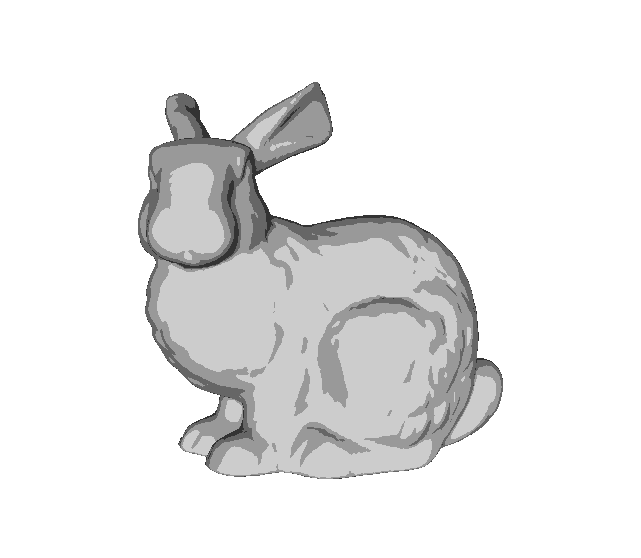
\includegraphics[width=0.7\textwidth]{toonShading.png}
\end{figure}
\newpage

\section*{4.3.1   Linear Depth Map }
The vertex will be somewhere between the near and the far planes on the z axis. So to get the depth, we need to subtract the near plane to the vertex's z component, while keeping in mind that the camera is looking in the negative. We then re-scale it between 0 and 1. So the depth is : $$depth = (-vertex.z - near)/(far - near)$$
\begin{figure}[h!]
\caption{Linear Depth Map}
  \centering
    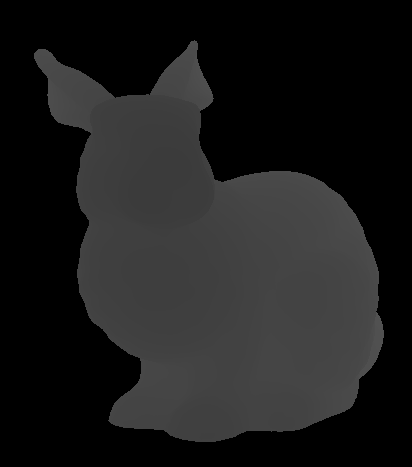
\includegraphics[width=0.7\textwidth]{linearDepthMap.png}
\end{figure}
\newpage

\section*{4.3.2   Edge Detection }
First, we define a method $value(int\ x, int\ y)$ to access the pixel we need for $Gx$ and $Gy$. We know to the pixel we are working on is $gl\_TexCoord[0].xy$, so its easy with the vector $(x,y)$ and $dx$, $dy$, to get the values of the pixels around it. We then hardcode the $Gx$ and $Gy$ and we set $gl\_FragColor$ to : $$1.0 - 10.0*sqrt(Gx*Gx + Gy*Gy)$$

\section*{4.4   Blending }
As said, this is easily done with a simple multiplication : $$gl_FragColor = cartoonColor * edgeColor$$
\begin{figure}[h!]
\caption{Blending}
  \centering
    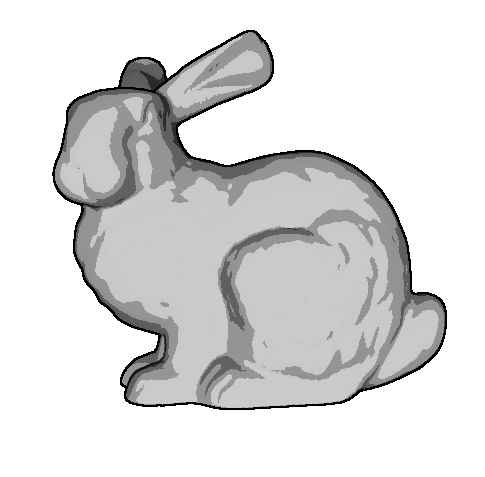
\includegraphics[width=0.7\textwidth]{blending.png}
\end{figure}

\end{document}